流量を比較するため,ランダムと渋滞,2種類の初期配置で実験した.
Fig.\ref{random_result}とFig.\ref{crowd_result}は2種類の初期配置での実験回数($x$軸)と
流量($y$軸)の関係図である.

点線がニューラルネットワークによる走行の結果,実線が$b=270,270$の感覚運動写像による走行の結果,
一点鎖線が$b=360,260$の感覚運動写像による走行の結果である.
ニューラルネットワークの流量が常に感覚運動写像の流量より高い,変動も少ない.

Fig.\ref{compare_result}はランダムの初期配置(実線)と渋滞の初期配置(一点鎖線)で
約5回の実験の流量平均値グラフである.
$x$軸はアルゴリズム種類,$y$軸は平均流量を表す.
この図からニューラルネットワークの平均流量は感覚運動写像より高くて,
異なる初期配置に対して平均流量が変わらない.
$b=270,270$の感覚運動写像の平均流量が初期配置によって差が観察されて,
それは実験の回数が不足と考られ,今後,実験の回数を増やす必要がある.


\vspace{-1mm}
\begin{figure}[!ht]
    \centering
    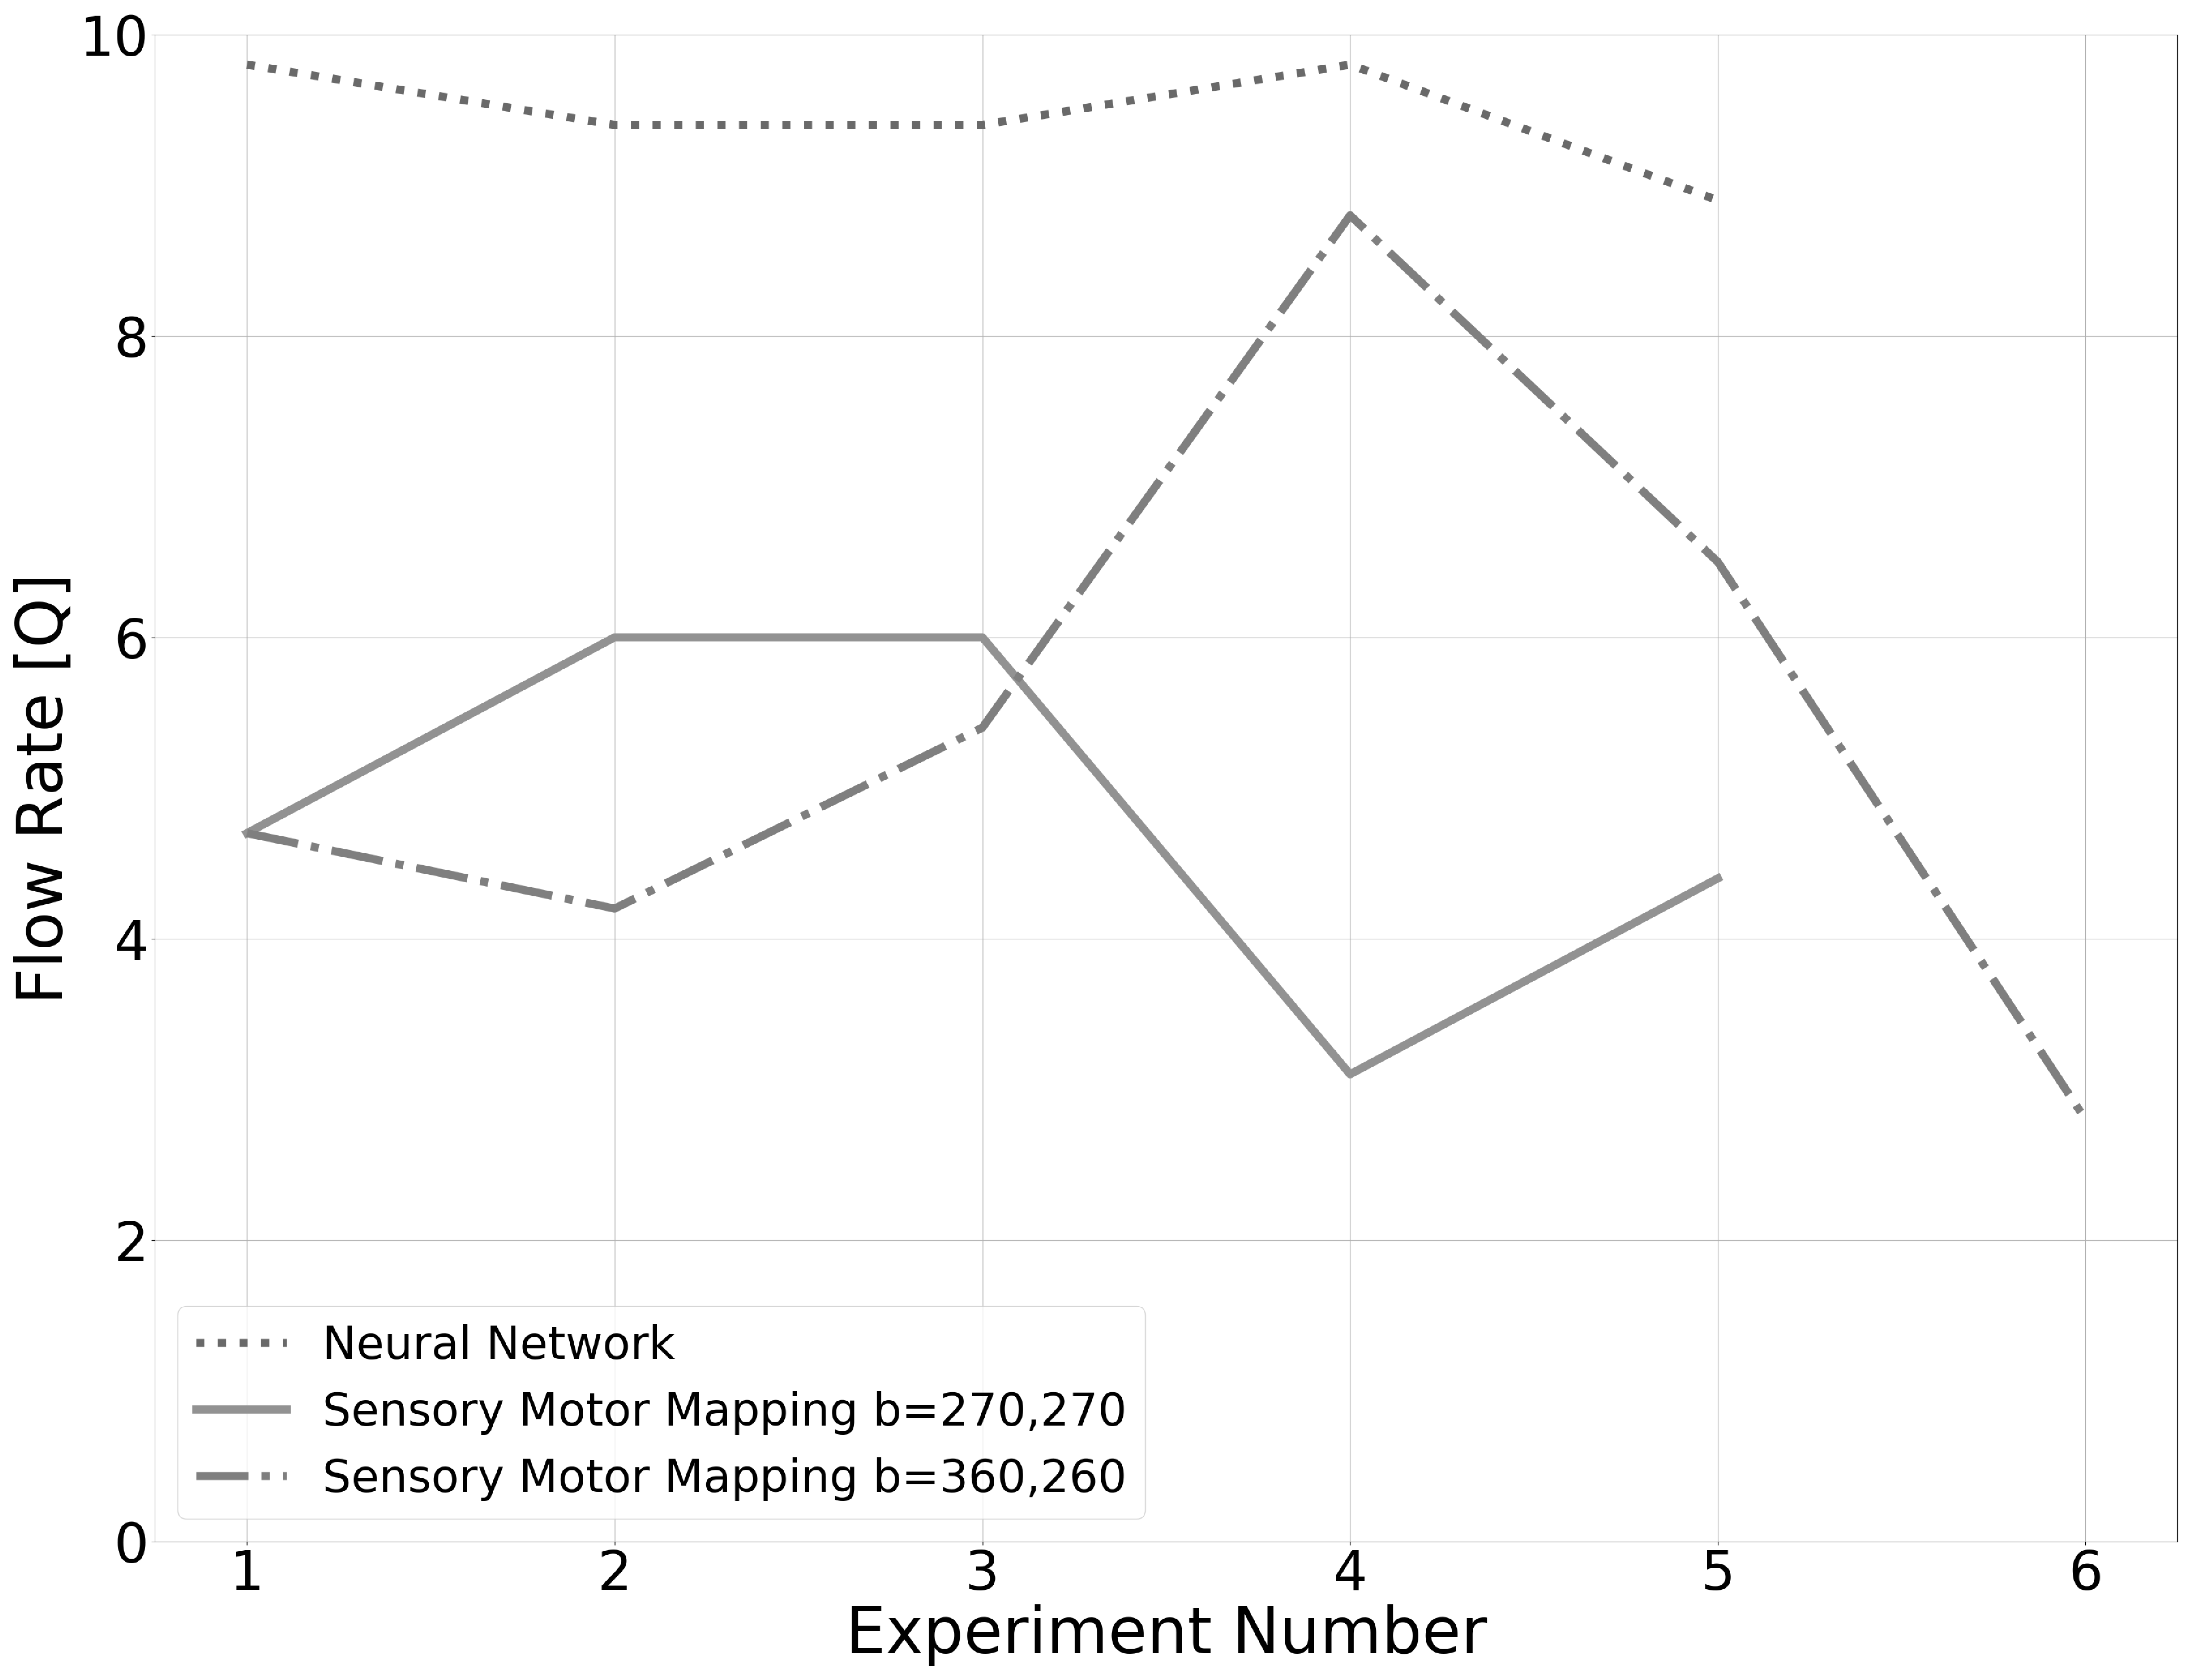
\includegraphics[width=0.9\linewidth]{result_diagrim_rand.eps}
    \caption{ランダムの初期配置で実験回数により流量の変化図}
    \label{random_result}
\end{figure}


\vspace{-1mm}
\begin{figure}[!ht]
    \centering
    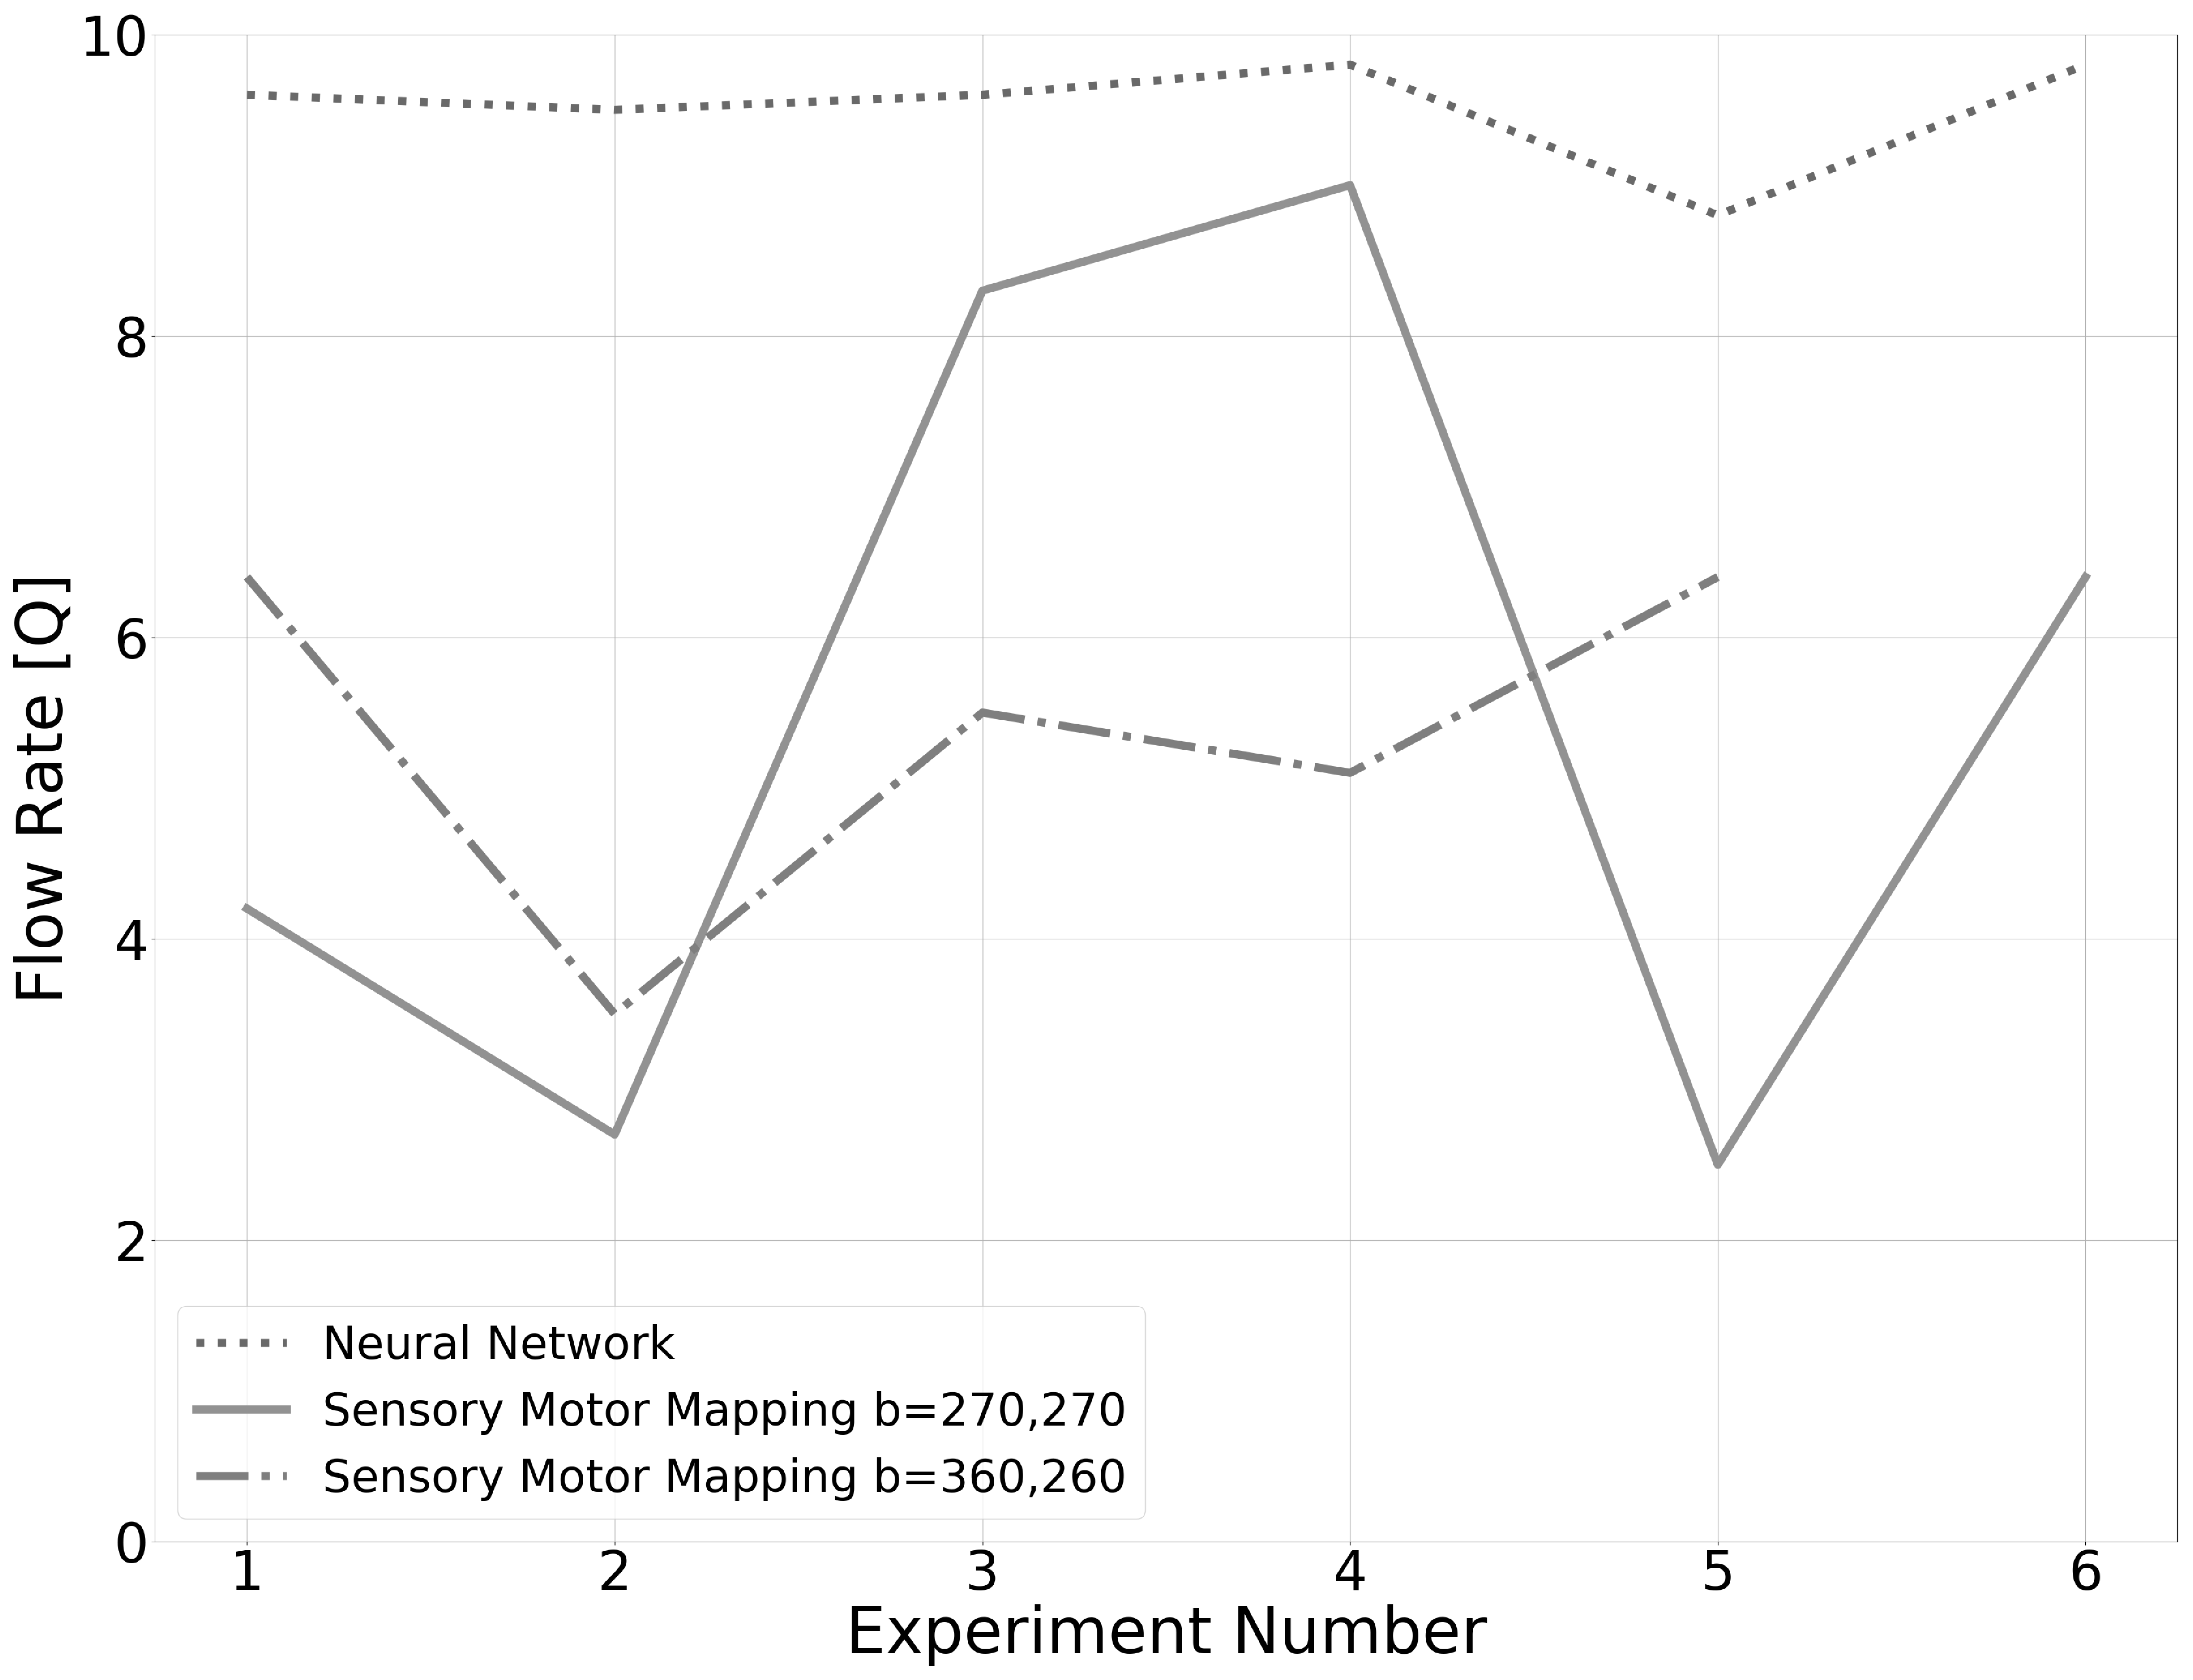
\includegraphics[width=0.9\linewidth]{result_diagrim_crow.eps}
    \caption{渋滞の初期配置で実験回数により流量の変化図}
    \label{crowd_result}
\end{figure}


\vspace{-1mm}
\begin{figure}[!ht]
    \centering
    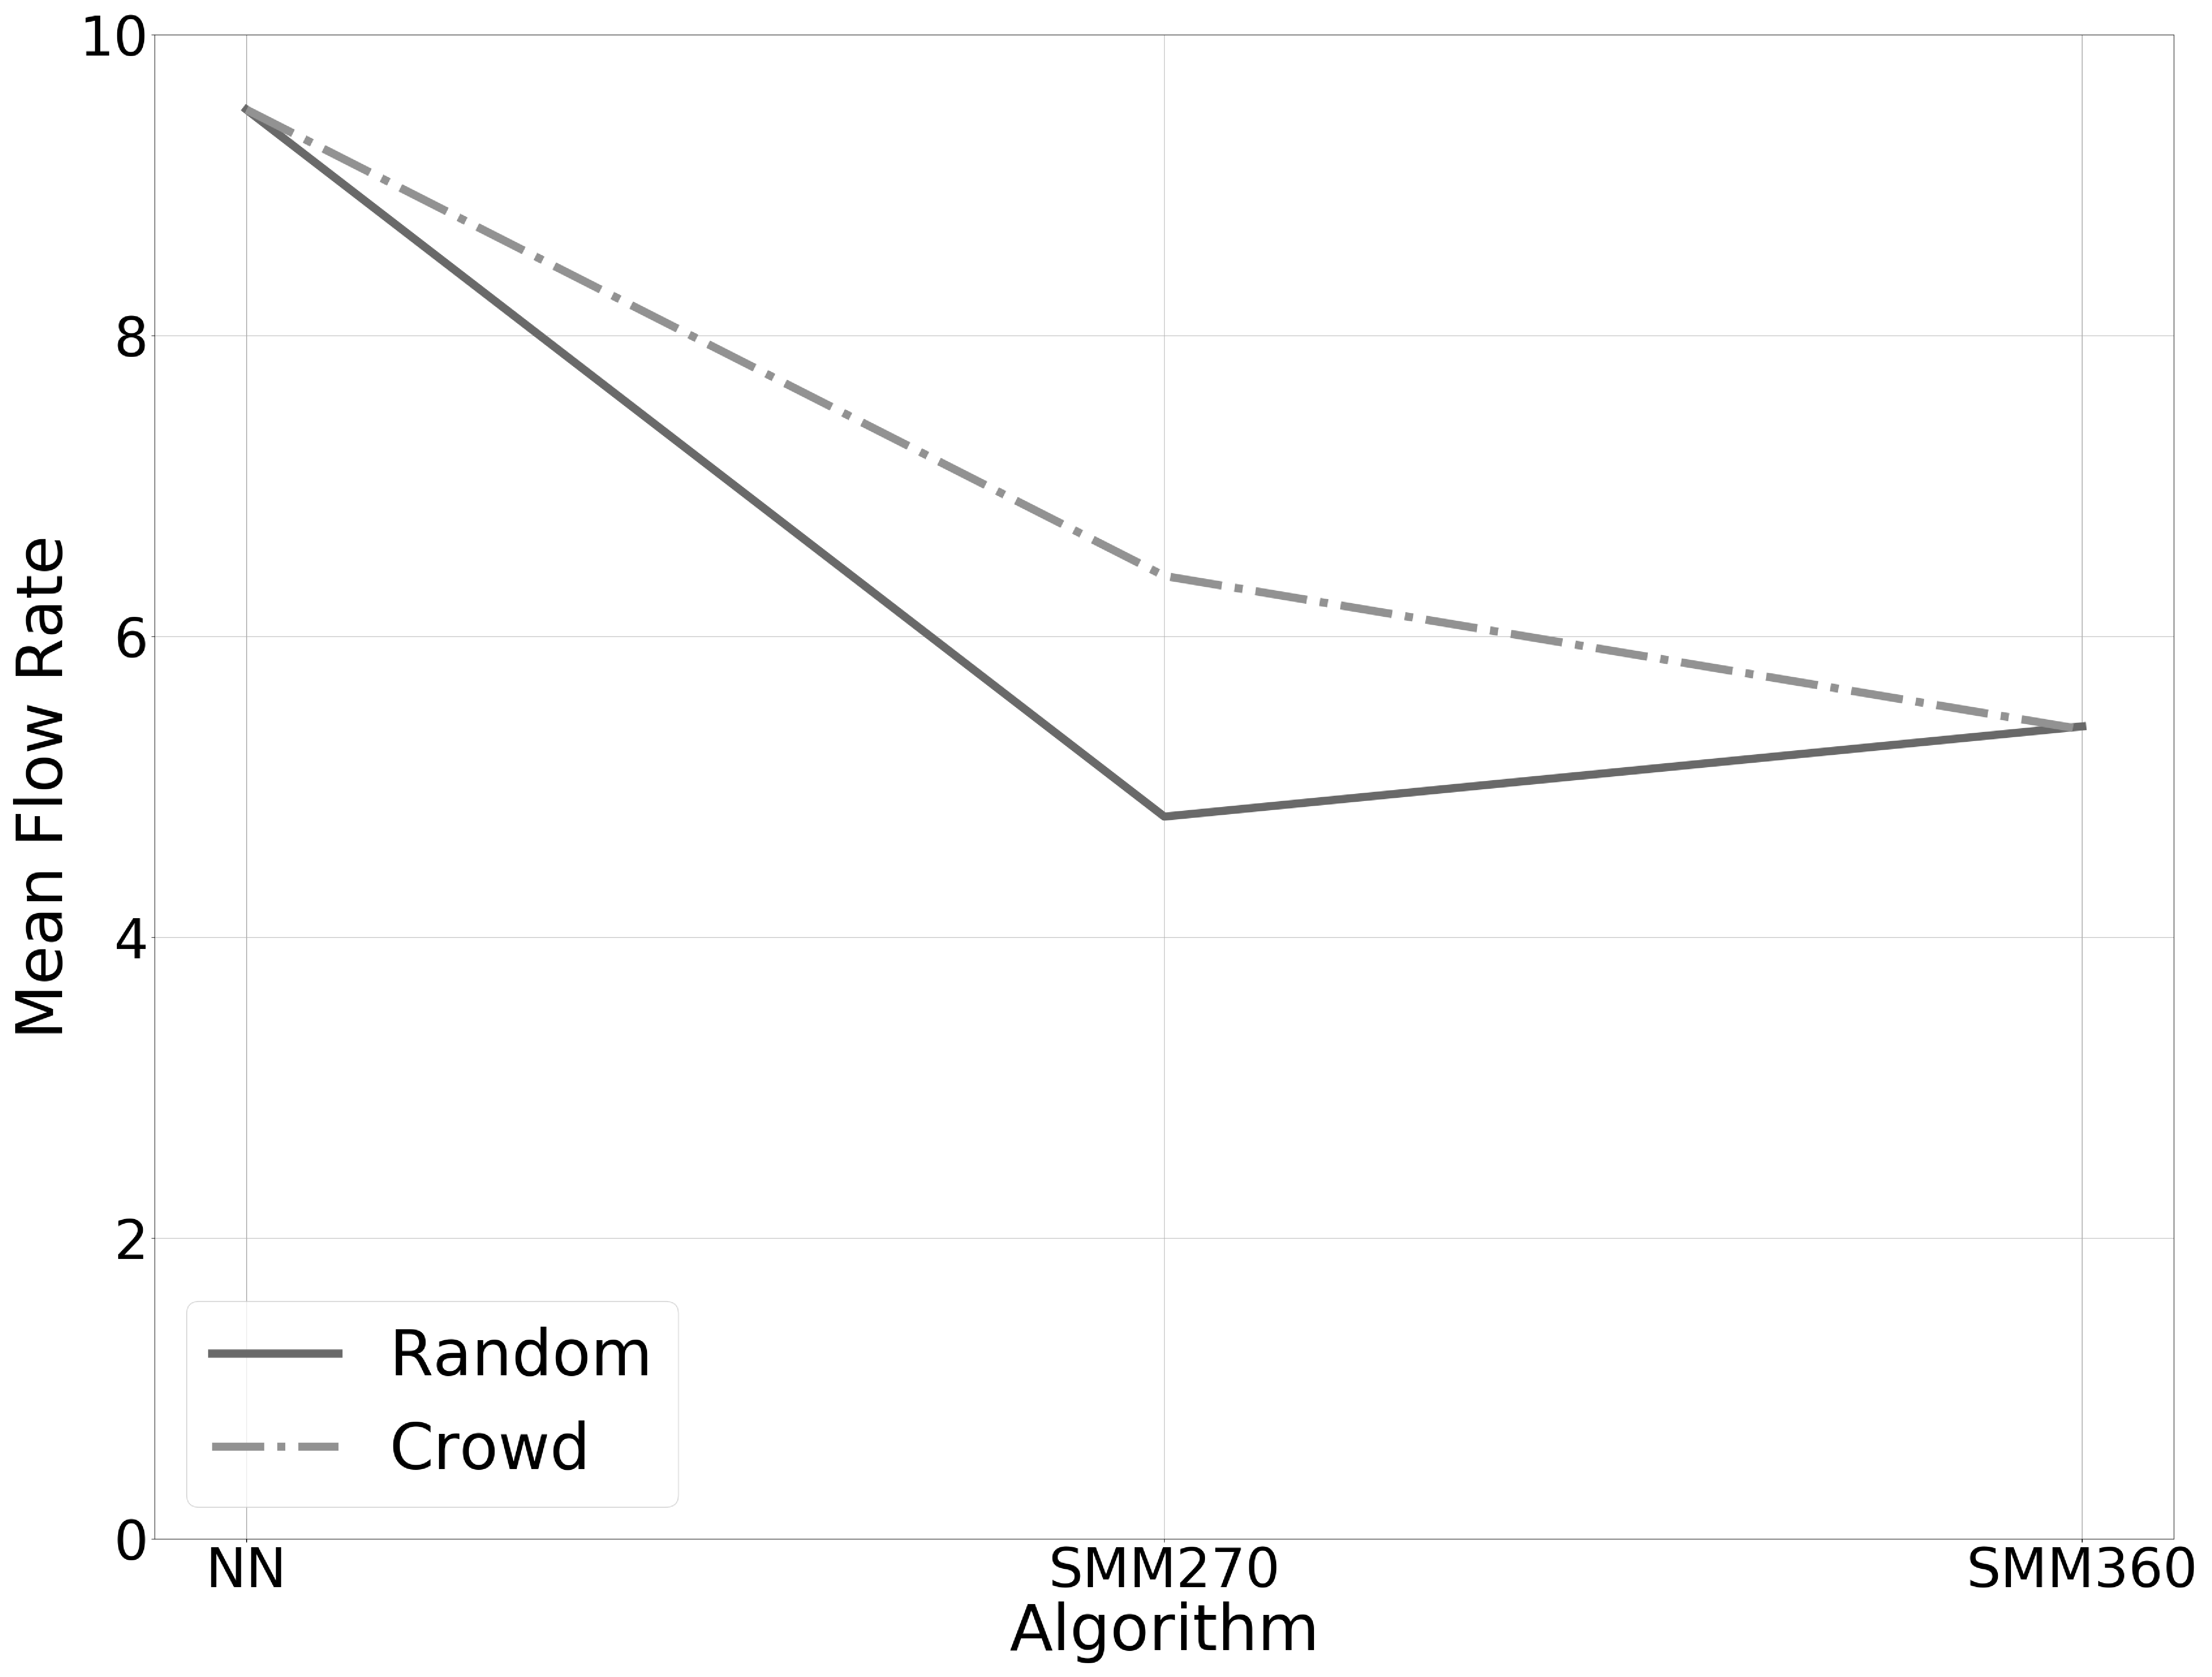
\includegraphics[width=0.9\linewidth]{mean_Q.eps}
    \caption{異なるアルゴリズムの平均流量の比較}
    \label{compare_result}
\end{figure}
